\section{Mathematical Uncertainty Theories}

As mentioned in \cite{uncertaintymeasuresbigpicture} and further detailed in chapters 2 and 3 of \cite{UncertaintySciences}, a theory of uncertainty typically consists of two elements:

\begin{romanenum}
    \item A mathematical representation that encodes uncertain states of the world and information about them.
    \item Mathematical operators and measures that enable reasoning about and combining uncertain information.
\end{romanenum}
\signal{No sé si compro eso de que rough sets tienen elementos precisos. Bueno sí, lo que pasa que tienes elementos precisos en clases de equivalencia. Tengo que revisar el ejemplo ese de granularity.}\\


\begin{figure}[ht]
    \hspace{2cm}
    \begin{tikzpicture}[>=stealth, font=\sffamily, align=center]
        % Define column x-positions.
        \def\xOne{-3}   % Column 1: Elements of Universal Set
        \def\xTwo{0}    % Column 2: Set (or event as a notion)
        \def\xThree{3}  % Column 3: Set Membership
        \def\xFour{6}   % Column 4: Example Theories
        
        % Use a common vertical center (here chosen as 0).
        \def\Bgap{0.75}
        
        % Column 2 vertical shifts.
        \def\CshiftA{2.25}
        \def\CshiftB{0.75}
        \def\CshiftC{-0.75}
        \def\CshiftD{-2.25}
        
        % Column 3 and Column 4 vertical shifts.
        \def\Dshiftone{5.25}
        \def\Dshifttwo{3.75}
        \def\Dshiftthree{2.25}
        \def\Dshiftfour{0.75}
        \def\Dshiftfive{-0.75}
        \def\Dshiftsix{-2.25}
        \def\Dshiftseven{-3.75}
        \def\Dshifteight{-5.25}
        
        % --------------------- Column 1 ---------------------
        % Small nodes
        \node (B1) at (\xOne, \Bgap)
              [rectangle, draw, fill=blue!10] {Precise\\ elements};
        \node (B2) at (\xOne, -\Bgap)
              [rectangle, draw, fill=blue!10] {Imprecise\\ elements};
              
        % Big rectangle in the background layer
        \begin{pgfonlayer}{background}
        \node[draw, thick, rounded corners,
              fill=gray!10,
              fit=(B1)(B2),
              inner sep=5pt,
              label={[align=center]above:\textbf{Elements}}
        ] (BoxB) {};
        \end{pgfonlayer}
        
        % --------------------- Column 2 ---------------------
        \node (C1) at (\xTwo, \CshiftA)
              [rectangle, draw, fill=blue!10] {Precise\\ set};
        \node (C2) at (\xTwo, \CshiftB)
              [rectangle, draw, fill=blue!10] {Imprecise\\ set};
        \node (C3) at (\xTwo, \CshiftC)
              [rectangle, draw, fill=blue!10] {Precise\\ set};
        \node (C4) at (\xTwo, \CshiftD)
              [rectangle, draw, fill=blue!10] {Imprecise\\ set};
        
        \begin{pgfonlayer}{background}
        \node[draw, thick, rounded corners,
              fill=gray!10,
              fit=(C1)(C4),
              inner sep=5pt,
              label={[align=center]above:\textbf{Set}}
        ] (BoxC) {};
        \end{pgfonlayer}
        
        % --------------------- Column 3 ---------------------
        \node (D1) at (\xThree, \Dshiftone)
              [rectangle, draw, fill=blue!10] {Binary};
        \node (D2) at (\xThree, \Dshifttwo)
              [rectangle, draw, fill=blue!10] {Non-\\binary};
        \node (D3) at (\xThree, \Dshiftthree)
              [rectangle, draw, fill=blue!10] {Binary};
        \node (D4) at (\xThree, \Dshiftfour)
              [rectangle, draw, fill=blue!10] {Non-\\binary};
        \node (D5) at (\xThree, \Dshiftfive)
              [rectangle, draw, fill=blue!10] {Binary};
        \node (D6) at (\xThree, \Dshiftsix)
              [rectangle, draw, fill=blue!10] {Non-\\binary};
        \node (D7) at (\xThree, \Dshiftseven)
              [rectangle, draw, fill=blue!10] {Binary};
        \node (D8) at (\xThree, \Dshifteight)
              [rectangle, draw, fill=blue!10] {Non-\\binary};
        
        \begin{pgfonlayer}{background}
        \node[draw, thick, rounded corners,
              fill=gray!10,
              fit=(D1)(D8),
              inner sep=5pt,
              label={[align=center]above:\textbf{Set Membership}}
        ] (BoxD) {};
        \end{pgfonlayer}
        
        % --------------------- Column 4 ---------------------
        \node (E1) at (\xFour, \Dshiftone)
              [rectangle, draw, fill=blue!10] {Crisp\\ sets};
        \node (E2) at (\xFour, \Dshifttwo)
              [rectangle, draw, fill=blue!10] {Rough\\ sets};
        \node (E3) at (\xFour, \Dshiftthree)
              [rectangle, draw, fill=blue!10] {Illogical};
        \node (E4) at (\xFour, \Dshiftfour)
              [rectangle, draw, fill=blue!10] {Fuzzy\\ sets};
        \node (E5) at (\xFour, \Dshiftfive)
              [rectangle, draw, fill=blue!10] {Illogical};
        \node (E6) at (\xFour, \Dshiftsix)
              [rectangle, draw, fill=blue!10] {Fuzzy\\ rough sets};
        \node (E7) at (\xFour, \Dshiftseven)
              [rectangle, draw, fill=blue!10] {Illogical};
        \node (E8) at (\xFour, \Dshifteight)
              [rectangle, draw, fill=blue!10] {Rough\\ fuzzy sets};
        
        \begin{pgfonlayer}{background}
        \node[draw, thick, rounded corners,
              fill=gray!10,
              fit=(E1)(E8),
              inner sep=5pt,
              label={[align=center]above:\textbf{Set Models}}
        ] (BoxE) {};
        \end{pgfonlayer}
        
        % --------------------- Edges ---------------------
        % Column 1 -> Column 2:
        \draw[->] (B1) -- (C1);
        \draw[->] (B1) -- (C2);
        \draw[->] (B2) -- (C3);
        \draw[->] (B2) -- (C4);
        
        % Column 2 -> Column 3:
        \draw[->] (C1) -- (D1);
        \draw[->] (C1) -- (D2);
        \draw[->] (C2) -- (D3);
        \draw[->] (C2) -- (D4);
        \draw[->] (C3) -- (D5);
        \draw[->] (C3) -- (D6);
        \draw[->] (C4) -- (D7);
        \draw[->] (C4) -- (D8);
        
        % Column 3 -> Column 4:
        \draw[->] (D1) -- (E1);
        \draw[->] (D2) -- (E2);
        \draw[->] (D3) -- (E3);
        \draw[->] (D4) -- (E4);
        \draw[->] (D5) -- (E5);
        \draw[->] (D6) -- (E6);
        \draw[->] (D7) -- (E7);
        \draw[->] (D8) -- (E8);
        
    \end{tikzpicture}
    \caption{Generalizations of crisp sets with different set models, showing increasing levels of expressivity for encoding data uncertainty.}
    \label{fig:Generalized_sets}
\end{figure}
























































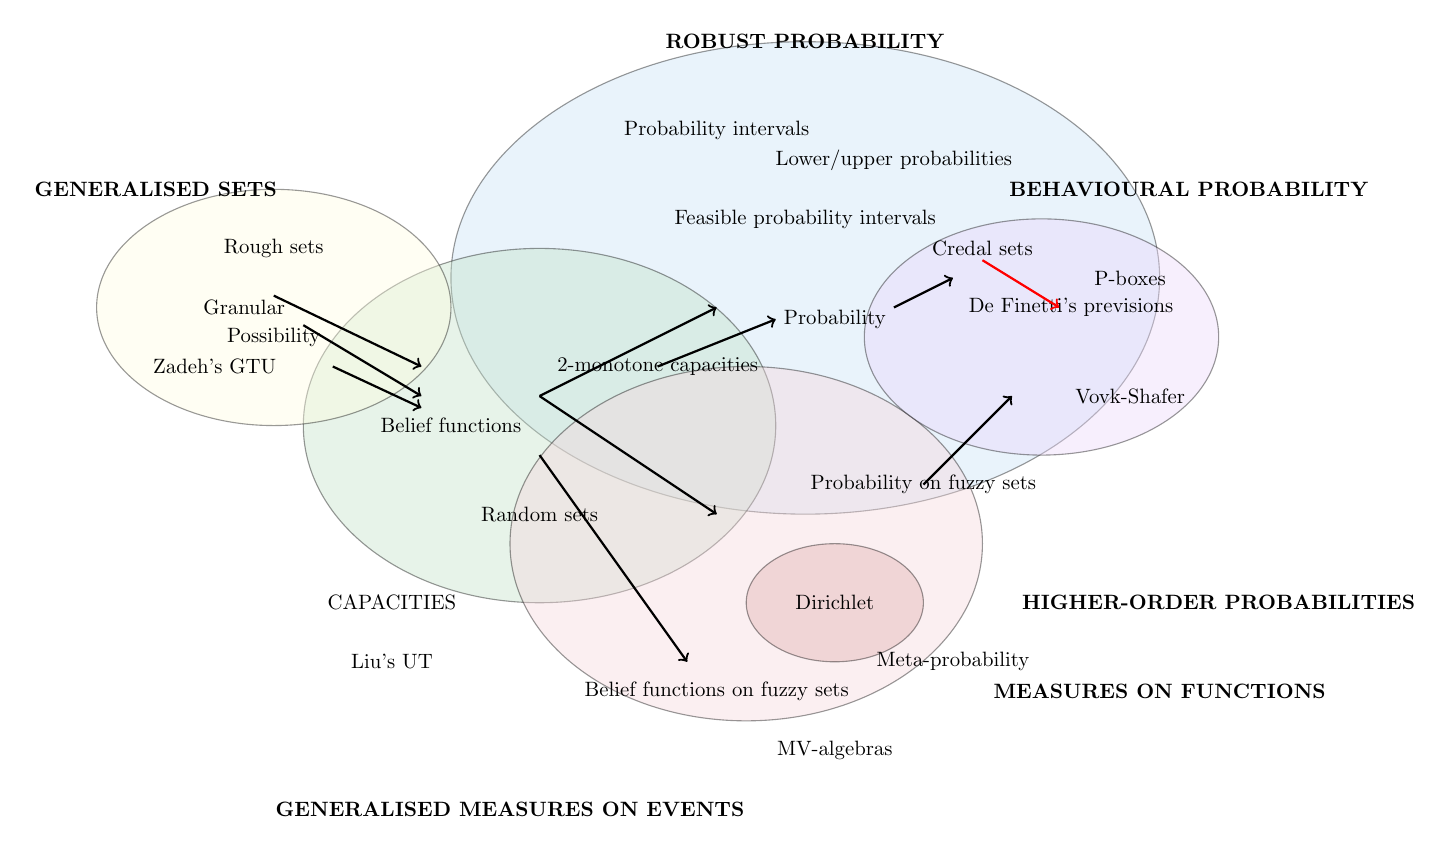
\begin{tikzpicture}[scale=0.75, every node/.style={scale=0.75}]

    % Colors
    \definecolor{bluearea}{RGB}{200,225,245}
    \definecolor{greenarea}{RGB}{195,225,200}
    \definecolor{yellowarea}{RGB}{255,253,225}
    \definecolor{redarea}{RGB}{245,215,220}
    \definecolor{purplearea}{RGB}{235,215,250}
    \definecolor{darkredarea}{RGB}{225,175,175}
    
    % Ellipses
    \draw[fill=bluearea,opacity=.4] (4,4.5) ellipse (6cm and 4cm);
    \draw[fill=greenarea,opacity=.4] (-0.5,2) ellipse (4cm and 3cm);
    \draw[fill=yellowarea,opacity=.4] (-5,4) ellipse (3cm and 2cm);
    \draw[fill=redarea,opacity=.4] (3,0) ellipse (4cm and 3cm);
    \draw[fill=purplearea,opacity=.4] (8,3.5) ellipse (3cm and 2cm);
    \draw[fill=darkredarea,opacity=.4] (4.5,-1) ellipse (1.5cm and 1cm);
    
    % Nodes (Texts)
    % Robust Probability
    \node at (4,8.5) {\textbf{ROBUST PROBABILITY}};
    \node at (2.5,7) {Probability intervals};
    \node at (5.5,6.5) {Lower/upper probabilities};
    \node at (4,5.5) {Feasible probability intervals};
    \node at (7,5) {Credal sets};
    \node at (9.5,4.5) {P-boxes};
    \node at (4.5,3.8) {Probability};
    
    % Generalised Sets
    \node at (-7,6) {\textbf{GENERALISED SETS}};
    \node at (-5,5) {Rough sets};
    \node at (-5.5,4) {Granular};
    \node at (-5,3.5) {Possibility};
    \node at (-6,3) {Zadeh's GTU};
    
    % Capacities
    \node at (-3,-1) {CAPACITIES};
    \node at (-2,2) {Belief functions};
    \node at (-0.5,0.5) {Random sets};
    \node at (-3,-2) {Liu's UT};
    \node at (1.5,3) {2-monotone capacities};
    
    % Behavioural Probability
    \node at (10.5,6) {\textbf{BEHAVIOURAL PROBABILITY}};
    \node at (8.5,4) {De Finetti's previsions};
    \node at (9.5,2.5) {Vovk-Shafer};
    
    % Measures on Functions
    \node at (10,-2.5) {\textbf{MEASURES ON FUNCTIONS}};
    \node at (6,1) {Probability on fuzzy sets};
    \node at (4.5,-1) {Dirichlet};
    \node at (6.5,-2) {Meta-probability};
    \node at (2.5,-2.5) {Belief functions on fuzzy sets};
    \node at (4.5, -3.5) {MV-algebras};
    
    \node at (11,-1) {\textbf{HIGHER-ORDER PROBABILITIES}};
    
    % Generalised measures on events
    \node at (-1,-4.5) {\textbf{GENERALISED MEASURES ON EVENTS}};
    
    % Arrows
    \draw[->,thick] (-4,3) -- (-2.5,2.3);
    \draw[->,thick] (-4.5,3.7) -- (-2.5,2.5);
    \draw[->,thick] (-5,4.2) -- (-2.5,3);
    \draw[->,thick] (-0.5,2.5) -- (2.5,4);
    \draw[->,thick] (-0.5,2.5) -- (2.5,0.5);
    \draw[->,thick] (-0.5,1.5) -- (2,-2);
    \draw[->,thick] (1.5,3) -- (3.5,3.8);
    \draw[->,thick] (5.5,4) -- (6.5,4.5);
    \draw[->,thick] (6,1) -- (7.5,2.5);
    \draw[->,thick,red] (7,4.8) -- (8.3,4);
    
    \end{tikzpicture}